\documentclass[]{article}
\usepackage{lmodern}
\usepackage{amssymb,amsmath}
\usepackage{ifxetex,ifluatex}
\usepackage{fixltx2e} % provides \textsubscript
\ifnum 0\ifxetex 1\fi\ifluatex 1\fi=0 % if pdftex
  \usepackage[T1]{fontenc}
  \usepackage[utf8]{inputenc}
\else % if luatex or xelatex
  \ifxetex
    \usepackage{mathspec}
  \else
    \usepackage{fontspec}
  \fi
  \defaultfontfeatures{Ligatures=TeX,Scale=MatchLowercase}
\fi
% use upquote if available, for straight quotes in verbatim environments
\IfFileExists{upquote.sty}{\usepackage{upquote}}{}
% use microtype if available
\IfFileExists{microtype.sty}{%
\usepackage{microtype}
\UseMicrotypeSet[protrusion]{basicmath} % disable protrusion for tt fonts
}{}
\usepackage[margin=1in]{geometry}
\usepackage{hyperref}
\hypersetup{unicode=true,
            pdftitle={Causal Inference Final Project: Effect of Smoking on 10-year Development of Coronary Heart Disease},
            pdfauthor={Bianca Doone, Michael Attah, Graham Casey Gibson, Daniel Saunders, Nutcha Wattanachit},
            pdfborder={0 0 0},
            breaklinks=true}
\urlstyle{same}  % don't use monospace font for urls
\usepackage{longtable,booktabs}
\usepackage{graphicx,grffile}
\makeatletter
\def\maxwidth{\ifdim\Gin@nat@width>\linewidth\linewidth\else\Gin@nat@width\fi}
\def\maxheight{\ifdim\Gin@nat@height>\textheight\textheight\else\Gin@nat@height\fi}
\makeatother
% Scale images if necessary, so that they will not overflow the page
% margins by default, and it is still possible to overwrite the defaults
% using explicit options in \includegraphics[width, height, ...]{}
\setkeys{Gin}{width=\maxwidth,height=\maxheight,keepaspectratio}
\IfFileExists{parskip.sty}{%
\usepackage{parskip}
}{% else
\setlength{\parindent}{0pt}
\setlength{\parskip}{6pt plus 2pt minus 1pt}
}
\setlength{\emergencystretch}{3em}  % prevent overfull lines
\providecommand{\tightlist}{%
  \setlength{\itemsep}{0pt}\setlength{\parskip}{0pt}}
\setcounter{secnumdepth}{0}
% Redefines (sub)paragraphs to behave more like sections
\ifx\paragraph\undefined\else
\let\oldparagraph\paragraph
\renewcommand{\paragraph}[1]{\oldparagraph{#1}\mbox{}}
\fi
\ifx\subparagraph\undefined\else
\let\oldsubparagraph\subparagraph
\renewcommand{\subparagraph}[1]{\oldsubparagraph{#1}\mbox{}}
\fi

%%% Use protect on footnotes to avoid problems with footnotes in titles
\let\rmarkdownfootnote\footnote%
\def\footnote{\protect\rmarkdownfootnote}

%%% Change title format to be more compact
\usepackage{titling}

% Create subtitle command for use in maketitle
\newcommand{\subtitle}[1]{
  \posttitle{
    \begin{center}\large#1\end{center}
    }
}

\setlength{\droptitle}{-2em}
  \title{Causal Inference Final Project: Effect of Smoking on 10-year Development
of Coronary Heart Disease}
  \pretitle{\vspace{\droptitle}\centering\huge}
  \posttitle{\par}
  \author{Bianca Doone, Michael Attah, Graham Casey Gibson, Daniel Saunders,
Nutcha Wattanachit}
  \preauthor{\centering\large\emph}
  \postauthor{\par}
  \predate{\centering\large\emph}
  \postdate{\par}
  \date{November 25, 2018}

\usepackage{float}

\begin{document}
\maketitle

\section{Background Story}\label{background-story}

Coronary heart disease (CHD) is the leading cause of death and serious
illness in the United States. The Framingham Heart Study's objective was
to identify the common factors or characteristics that contribute to CHD
by following its development over time in a large group of participants
who had not yet developed overt symptoms of CHD or suffered a heart
attack or stroke.

The researchers recruited 5,209 men and women between the ages of 30 and
70 from Framingham, Massachusetts, and began the first round of
extensive physical examinations and lifestyle interviews that they would
later analyze for common patterns related to CHD development. Over the
years, careful monitoring of the Framingham Study population has led to
the identification of the major CHD risk factors -- high blood pressure,
high blood cholesterol, smoking, obesity, diabetes, and physical
inactivity. We are interested how the extent of smoking affects the
development of CHD, specifically, it is not immediately obvious whether
smoking 5 cigarettes per day affects the development of CHD differently
than smoking 15 cigarettes per day does.

\section{Causal Roadmap}\label{causal-roadmap}

\subsection{Step 0: Specify the Scientific
Question}\label{step-0-specify-the-scientific-question}

What is the effect of smoking on the ten-year development of Coronary
Heart Disease?

\paragraph{Target population}\label{target-population}

The target population is white middle-class men and women aged 30 to 70
in the US.

The sameple in this study is white middle-class men and women aged 30 to
70 (at baseline) in Framingham, Massachusetts. The importance of the
major CHD risk factors identified in this group have been shown in other
studies to apply almost universally, even though the patterns of
distribution may vary. Thus, we are willing to generalize to the target
population.

\subsection{Step 1: Specify a Causal
Model}\label{step-1-specify-a-causal-model}

\begin{itemize}
\item
  Endogenous nodes: \(X = (W,Z,A,Y)\), where
\item
  \(W\) is age, gender, education
\item
  \(Z\) is blood pressure (systolic and diastolic), total Cholesterol,
  prevalence of hypertension, prevalence of stroke, heart rate, BMI,
  Diabetes prevalence
\item
  \(A\) is the number of cigarettes smoked per days
\item
  \(Y\) is the ten-year development of coronary heart disease (CHD).
\item
  Exogenous nodes: \(U = (U_{W}, U_{Z}, U_A , U_Y) \sim \mathbb{P}_U\).
  We make no assumptions about the distribution \(\mathbb{P}_U\).
\item
  Structural equations \(F\): \[
  \begin{aligned}
  W &\leftarrow  f_W (U_W) \\
  Z  &\leftarrow  f_Z (W, A, U_Z) \\
  A  &\leftarrow  f_A (W, U_A) \\
  Y  &\leftarrow  f_Y (W, Z, A, U_Y) \\
  \end{aligned}
  \]
\end{itemize}

There are no exclusion restrictions or assumptions about functional
form.

\paragraph{Causal Graph}\label{causal-graph}

\begin{figure}[H]

{\centering 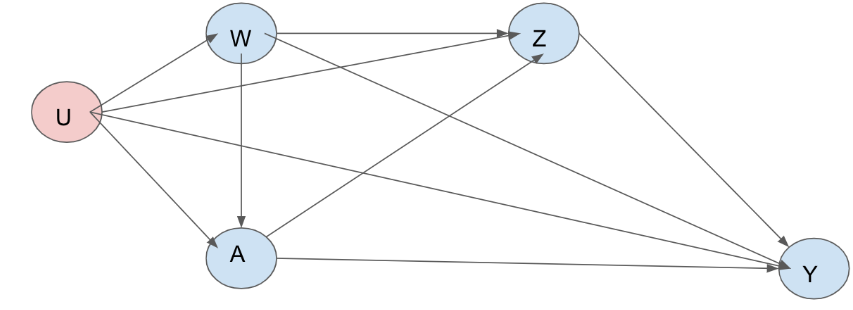
\includegraphics[width=0.9\linewidth]{./dags/dag_causal} 

}

\caption{Causal Graph for the SCM}\label{fig:fig1}
\end{figure}

\subsection{Step 2: Counterfactuals \& Causal
Parameter}\label{step-2-counterfactuals-causal-parameter}

\paragraph{Causal Parameter}\label{causal-parameter}

\[{\Psi^*}^{i}(\mathbb{P}^*)=\mathbb{E}^*[Y_i]\ \ \ i\in \{1,2,3,4\}\]
where \(i\) represent the bin of cigarettes smoked per day. \(Y_i\)
denotes the counterfactual outcome (the ten-year development of
cardiovascular disease), if possibly contrary to fact, a person's number
of cigarettes smoked per day is within \(i^{th}\) bin.

\subsection{Step 3. Specify your observed data and its link to the
causal
model}\label{step-3.-specify-your-observed-data-and-its-link-to-the-causal-model}

The dataset is adapted from Framingham Heart Study. We assume that
Gender, Age, Education, and Number of Cigarettes per Day (\(A\)) were
collected in a questionnaire at baseline. Then, BMI, Diabetes Status,
Prevalence of Stroke, Prevalence of Hypertension, Indication of Blood
Pressure Medication, Total Cholesterol Level, Blood Pressure, and Heart
Rate were all collected after the questionnaire at a doctor's office.
Our outcome, Coronary Heart Disease, is collected at a 10-year follow
up. Note that this is unlike the original study. We assume our observed
data were generated by sampling \(n\) from a system described by our
structural causal model, so we have \(n = 4211\) copies of
\(O\overset{i.i.d}\sim \mathbb{P}_O\). We place no restrictions on the
statistical model \(\mathcal{M}\), which is thereby non-parametric. BMI
was binned using guidelines from the World Health Organization. Total
Cholesterol was binned using guidelines from the National Heart, Lung
and Blood Institute (NHLBI). Table 1 below shows the counts for each
variable in each bin of the exposure, as well as a \(\chi^2\)-test of
independence.

\begin{longtable}[]{@{}lllllll@{}}
\caption{Number of Observations in Each Bin}\tabularnewline
\toprule
& Level & {[}0,1) & {[}1,10) & {[}10,19) & {[}20,70{]} &
p\tabularnewline
\midrule
\endfirsthead
\toprule
& Level & {[}0,1) & {[}1,10) & {[}10,19) & {[}20,70{]} &
p\tabularnewline
\midrule
\endhead
n & & 2089 & 471 & 380 & 1168 &\tabularnewline
diabetes (\%) & 0 & 2022 ( 96.8) & 463 ( 98.3) & 372 ( 97.9) & 1145 (
98.0) & 0.079\tabularnewline
& 1 & 67 ( 3.2) & 8 ( 1.7) & 8 ( 2.1) & 23 ( 2.0) &\tabularnewline
prevalentStroke (\%) & 0 & 2071 ( 99.1) & 469 ( 99.6) & 377 ( 99.2) &
1166 ( 99.8) & 0.095\tabularnewline
& 1 & 18 ( 0.9) & 2 ( 0.4) & 3 ( 0.8) & 2 ( 0.2) &\tabularnewline
prevalentHyp (\%) & 0 & 1337 ( 64.0) & 338 ( 71.8) & 293 ( 77.1) & 860 (
73.6) & \textless{}0.001\tabularnewline
& 1 & 752 ( 36.0) & 133 ( 28.2) & 87 ( 22.9) & 308 ( 26.4)
&\tabularnewline
age (\%) & {[}32, 42) & 363 ( 17.4) & 117 ( 24.8) & 110 ( 28.9) & 309 (
26.5) & \textless{}0.001\tabularnewline
& {[}42, 49) & 464 ( 22.2) & 137 ( 29.1) & 125 ( 32.9) & 401 ( 34.3)
&\tabularnewline
& {[}49, 56) & 527 ( 25.2) & 97 ( 20.6) & 71 ( 18.7) & 254 ( 21.7)
&\tabularnewline
& {[}56, 70{]} & 735 ( 35.2) & 120 ( 25.5) & 74 ( 19.5) & 204 ( 17.5)
&\tabularnewline
education (\%) & 1 & 915 ( 43.8) & 188 ( 39.9) & 137 ( 36.1) & 470 (
40.2) & 0.003\tabularnewline
& 2 & 574 ( 27.5) & 150 ( 31.8) & 121 ( 31.8) & 399 ( 34.2)
&\tabularnewline
& 3 & 367 ( 17.6) & 76 ( 16.1) & 71 ( 18.7) & 170 ( 14.6)
&\tabularnewline
& 4 & 233 ( 11.2) & 57 ( 12.1) & 51 ( 13.4) & 129 ( 11.0)
&\tabularnewline
BP (\%) & 0 & 1139 ( 54.5) & 267 ( 56.7) & 211 ( 55.5) & 701 ( 60.0) &
0.025\tabularnewline
& 1 & 950 ( 45.5) & 204 ( 43.3) & 169 ( 44.5) & 467 ( 40.0)
&\tabularnewline
totChol (\%) & {[}0, 200) & 386 ( 18.6) & 108 ( 23.4) & 84 ( 22.3) & 227
( 19.7) & 0.004\tabularnewline
& {[}200, 240) & 723 ( 34.9) & 151 ( 32.7) & 157 ( 41.8) & 401 ( 34.9)
&\tabularnewline
& {[}240, 600{]} & 962 ( 46.5) & 203 ( 43.9) & 135 ( 35.9) & 522 ( 45.4)
&\tabularnewline
gender (\%) & 0 & 1400 ( 67.0) & 346 ( 73.5) & 222 ( 58.4) & 386 ( 33.0)
& \textless{}0.001\tabularnewline
& 1 & 689 ( 33.0) & 125 ( 26.5) & 158 ( 41.6) & 782 ( 67.0)
&\tabularnewline
bmi (\%) & {[}0, 18.5) & 19 ( 0.9) & 13 ( 2.8) & 7 ( 1.8) & 17 ( 1.5) &
\textless{}0.001\tabularnewline
& {[}18.5, 25) & 785 ( 37.8) & 245 ( 52.2) & 225 ( 59.2) & 568 ( 48.8)
&\tabularnewline
& {[}25, 30) & 940 ( 45.3) & 170 ( 36.2) & 117 ( 30.8) & 467 ( 40.1)
&\tabularnewline
& {[}30, 56.8{]} & 333 ( 16.0) & 41 ( 8.7) & 31 ( 8.2) & 112 ( 9.6)
&\tabularnewline
heartRate (\%) & {[}0, 60) & 122 ( 5.8) & 27 ( 5.7) & 19 ( 5.0) & 28 (
2.4) & \textless{}0.001\tabularnewline
& {[}60, 143{]} & 1967 ( 94.2) & 444 ( 94.3) & 360 ( 95.0) & 1140 (
97.6) &\tabularnewline
CHD (\%) & 0 & 1784 ( 85.4) & 420 ( 89.2) & 320 ( 84.2) & 958 ( 82.0) &
0.002\tabularnewline
& 1 & 305 ( 14.6) & 51 ( 10.8) & 60 ( 15.8) & 210 ( 18.0)
&\tabularnewline
\bottomrule
\end{longtable}

\subsection{Step 4. Identifiability}\label{step-4.-identifiability}

Since we made no independence assumptions on our exogenous background
factors, we will need to make additional independence assumptions for
identifiability. For the target causal parameter in the SCM
\(\mathcal{M^*}\) to be identified from the observed data distribution,
we need to make a randomization and a positivity assumption.

\paragraph{1) Randomization Assumption}\label{randomization-assumption}

We could assume that all unmeasured background factors in our SCM are
independent, which is sufficient, but not minimally sufficient. In the
augmented/working SCM (\(\mathcal{M^{**}}\)) that we selected, the
unmeasured background factor of \(A\) (cigarettes smoked per day) is
independent of the unmeasured background factor of \(Y\) (10yr CHD), the
unmeasured background factor of \(W\) (baseline age, gender, education,
diabetes, BMI), and the unmeasured background factor of \(Z\)
(prevalence of stroke, hypertension, blood pressure, blood pressure
medication, heart rate). Thus, conditional on \(W\), the counterfactual
outcome is independent of the observed treatment: \(Y \perp A|W\).

Since \(W\),\(Z\), and \(Y\) include SES and biological factors that
affect human health, we aviod assuming independence between their
unmeasured background factors. Thus, we consider it is more plausible to
make the indepedence assumptions listed. We do not adjust the mediator
\(Z\) to avoid opening a backdoor path. Under \(M^{**}\), the backdoor
criterion holds conditional on \(W\). Additional data on factors that
affect heath status and determinants could help with identifiability,
but those factors are not well-understood.

\begin{figure}[H]

{\centering 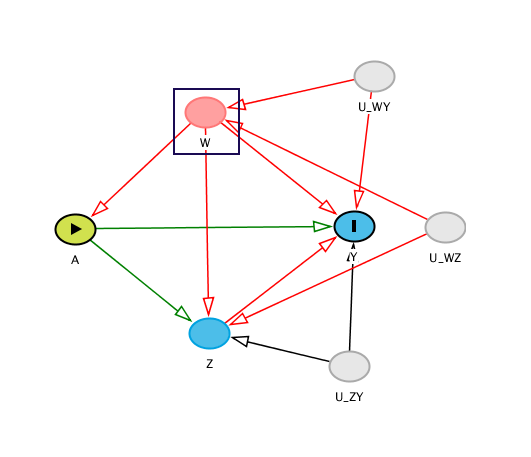
\includegraphics[width=0.65\linewidth]{./dags/augmented_dag} 

}

\caption{Causal Graph for an augmented SCM}\label{fig:fig2}
\end{figure}

\[U_A\perp U_Y,U_A\perp U_W,U_A\perp U_Z\]

\paragraph{2) Positivity Assumption}\label{positivity-assumption}

There must be a positive probability of each treatment condition within
each possible strata of \(W\). We need a positive probability of
cigarettes smoked per day in bin \(i\) for each strata of \(W\).

\[
\begin{aligned}
min_{i\in A}\mathbb{P}_0(A=i|W=w)>0\\
\text{for all}\ w \ \text{for which } 
\mathbb{P}_0(W = w) \geq 0
\end{aligned}
\]

where \(i\) denote the index of a bin of \(A\).

We are concerned about a positivity assumption violation since binning
covatiates could make particular stratas of \(W\) have low probabilities
of smoking certain numbers of cigarettes per day, especially a bin with
high numbers of cigarettes smoked per day. We can informally check for a
positivity assumption violation from tables of \(A\) given a strata of
\(W\).

From the table from one of the stratas of \(W\) below, we can see that
we have no female who smokes 10 to less than 20 cigarettes per day with
missing education level in the age ranges {[}42, 49) and {[}56, 70{]}
respectively. Thus, we have some sparsity issue which could affect the
estimator performance, particularly the inverse probability of treatment
weighting (IPTW).

\begin{table}[h!]
\centering
\caption{Table for Gender = 0 (Female), cigsPerDay (A) = [10,20) }
\small
\begin{tabular}{|l|l|l|l|l|l|}
\hline
Strata & Education: 1 & Education: 2 & Education: 3 & Education: 4 & Education: NA \\ \hline
Age: [32, 42) & 16 & 26 & 16 & 11 &  1 \\ \hline
Age: [42, 49) & 23 & 33 & 17 & 10 &  0 \\ \hline
Age: [49, 56) & 16 & 12 & 8 & 2 &  3  \\ \hline
Age: [56, 70] & 15 & 11 & 5 & 1 &  0  \\ \hline
\end{tabular}
\end{table}

We also investigated the treatment mechanism by calculating the
predicted probability of each bin of \(A\) (the number of cigarettes
smoked per day) given a strata of \(W\):

\begin{longtable}[]{@{}lrrr@{}}
\caption{Predicted Probabilities of A for each Strata of
W}\tabularnewline
\toprule
& Min & Mean & Max\tabularnewline
\midrule
\endfirsthead
\toprule
& Min & Mean & Max\tabularnewline
\midrule
\endhead
0 cigarettes per day & 0.2853671 & 0.5085200 & 0.7440546\tabularnewline
{[}1,10) cigarettes per day & 0.0612951 & 0.1146543 &
0.1733320\tabularnewline
{[}10,19) cigarettes per day & 0.0592084 & 0.0925024 &
0.1428044\tabularnewline
{[}20,70{]} cigarettes per day & 0.0765399 & 0.2843233 &
0.5630990\tabularnewline
\bottomrule
\end{longtable}

From the table's minimum probability column, we can see that some
stratas of \(W\) have relatively low probabilities for the number of
cigarettes smoked per day in the 2nd, 3rd, and 4th bin, which would
results in those stratas having high weights in the IPTW estimator.
However, the probabilities are not close to zero. Therefore, we do not
have a practical violation of positivity assumption. Theoretically,
randomizing the number of cigarettes smoked per day could rid of
positivity assumption violation concerns, but it is not feasible.

\subsection{Step 5. Statistical Model and
Estimand}\label{step-5.-statistical-model-and-estimand}

The target parameter of \(\mathbb{P}_0\), which equals the causal
parameter in the augmented causal model \(\mathcal{M}^{**}\) is given by
the G-Computation formula:

\[
\begin{aligned}
\Psi_0(\mathbb{P}^i_0)&=\mathbb{E}_0[\mathbb{E}_0[Y|A= i,W=w]]\\
&= \sum_w\mathbb{E}_0[Y|A=i,W=w]*\mathbb{P}_0(W=w)
\end{aligned}
\] where \(i\) represent the bin of cigarettes smoked per day.

\subsection{Step 6. Estimation}\label{step-6.-estimation}

In order to estimate the causal effect of smoking on risk of CHD we
evaluate 6 separate estimators. The first is a classical estimate made
by logistic regression. The second is a simple subsitution estimator.
The next 3 are variations of the IPTW estimator and finally we evaluate
the TMLE estimator. All confidence intervals presented below are based
on \(1,000\) bootstrap samples, expect in the case of IPTW-IC where the
influence curve confidence intervals were obtained and in the case of
the classical GLM where theoretical CI were obtained. This was done
mostly to evaluate the performance of the bootstrap confidence agains
the theoretical confidence derived from the influence curve.

\subsubsection{Classical Model Based on
Chi-Squared}\label{classical-model-based-on-chi-squared}

In order to comapre the causal based estimators to traditional
statistics, we first fit a generalized linear model as follows.

\[logit(CHD) \sim \beta_0 + \beta_1*\text{education} + \beta_2*\text{age} +\beta_3*\text{total cholesterol} \]

\[+ \beta_4*\text{prevelant Hyp} + \beta_5*\text{BP} + \beta_6*\text{diabetes} + \epsilon\]
Here we have included all variables that were considered signficiantly
correlated with the outcome under the \(\chi^2\) test of independence.
This includes conditioning on mediator variables such as a diabetes, a
distinct diference from the causal models presented below. In order to
obtain an estimate of \(E(Y | A=a_i)\) we simply call the predict method
on our existing data (with no specific intervention) and average the
results.

\subsubsection{Simple Substitution}\label{simple-substitution}

In order to evaluate our causal estimate we implemented a non-parametric
simple substiution estimator for the conditional mean outcome. We used a
saturated logistic regression model that included all possible
interaction terms to model \(P(Y | A=a ,W)\). The resulting estimator is
given for the \(i^{th}\) bin by

\[ SS^{i} = E_o[E_o[Y | A=a_i,W]]\]

Confidence intervals were obtained via the bootstrap.

\subsubsection{IPTW}\label{iptw}

In order to evaluate our causal estimate we examined three variations on
the traditional IPTW estimator as follows.

For the \(i^{th}\) bin:

\[IPTW^i = \frac{1}{n_i} \sum_{j}^{n_i} Y\frac{ \mathbb{I} [A = i]}{P(A = i | W)}\]
We evaluated 1) simple IPTW 2) horvitz thompson weighted IPTW 3) IPTW
with variance derived from influence curve calculations.

\begin{figure}[H]

{\centering \includegraphics[width=0.9\linewidth]{framingham_files/figure-latex/fig3-1} 

}

\caption{Distribution of Weights}\label{fig:fig3}
\end{figure}

We can see from the weight histograms that bin 2 has the largest
discrepency in the weighting. This may help explain why we see a
protective effect of smoking in bin 2.

\subsubsection{TMLE}\label{tmle}

Finally we examined our causal estimate under targeted maximum
likelihood. In our superlearner library we evaluated 4 candidate
algorithms

\[\{\text{Sl.glmnet,SL.randomForest,SL.nnet,SL.earth\}}\] Both our
estimate for the conditional mean outcome and the treatment probability
were obtained from superlearner.

\begin{figure}[H]

{\centering \includegraphics[width=0.8\linewidth]{framingham_files/figure-latex/fig4-1} 

}

\caption{Confidence Intervals for Estimators}\label{fig:fig4}
\end{figure}

As we can see from Fig. 4 the glm estimate is highly variable compared
with the causal estimator. In addition we see that estimates given by
the horvitz thompson IPTW and simple IPTW are quite comaprable with only
slightly smaller confidence intervals under horvitz thompson, as to be
expected. The theoertical intervals obtained from the influence curve
for IPTW were slightly larger than the bootstrap intervals, which might
be an issue with the bootstrap sample size. Finally, the estimates from
TMLE were conservative with respect to the other estimators \#\# Step 7.
Result Interpretation

\subsubsection{Statistical}\label{statistical}

From the estimation of our statistical model \(\mathcal{M}\), we found
that the probability of developing coronary heart disease increases as
the binned exposure (\texttt{cigsPerDay}) increases from, standardadized
to the distribution of baseline covariates \(W\). However, in bin \#2,
corresponding to \texttt{cigsPerDay} \(\in [1, 10)\), we found what
seems to be a ``protective'' effect, in which smoking less than a pack
of cigarettes as day is associated with a lower risk of CHD than not
smoking at all. The difference risk in this bin is estimated at around
0.10-0.11, compared with . We argue that this may be due to
\textit{non-differential misclassification}, since participants may have
not self-reported smoking due to the negative stigma associated with it.
For \texttt{cigsPerDay} \(\geq\) 20, the probability of CHD plateaus
near 0.2 (for the conditional mean outcome and IPTW estimators) and 0.16
(for TMLE).

\subsubsection{Counterfactual}\label{counterfactual}

The estimated effect of the exposure is the counterfactual probability
of developiong coronary heart disease in 10 years under the exposure
category \texttt{cigsPerDay} (\(A_i, i \in \{1, 2, 3, 4 \}\)), with the
assumptions that conditioning on the baseline covariates \(W\) (age,
sex, \& education) and assumpting certain independence assumptions
satisfies the backdoor criterion, and said independence assumptions and
positivity holds. The observed general increase in estimated risk of CHD
as the (binned) exposure increases is certainly plausible; however, the
estimated reduction in risk of CHD for \texttt{cigsPerDay}
\(\in [1, 10)\) is less plausible, again perhaps due to biased data from
non-differential misclassification on the exposure, or could in fact be
evidence for a protective effect of low degrees of smoking on risk of
CHD.

\subsubsection{Limitations}\label{limitations}

It is not likely that our target causal parameter is identifiable due to
violations of the chosen independence assumptions, and thus our
counterfactual estimation should not be accepted without some healthy
skepticism. Many unmeasured confounders are possible, including
pre-existing medical conditions not considered by the Framingham Heart
Study patient surveys, diet and exercise habits, family history, genetic
factors, and more. Future studies might expand the set of measured
variables to include such information. As mentioned, we are also
concerned about potential issues with reporting bias in the data.
Finally, we did not have access to time-varying aspects of the data;
e.g., smoking habits and biomarkers before or after baseline
measurements were taken, many of which could contain information
relevant to prediction of CHD outcomes.

\begin{figure}[H]

{\centering 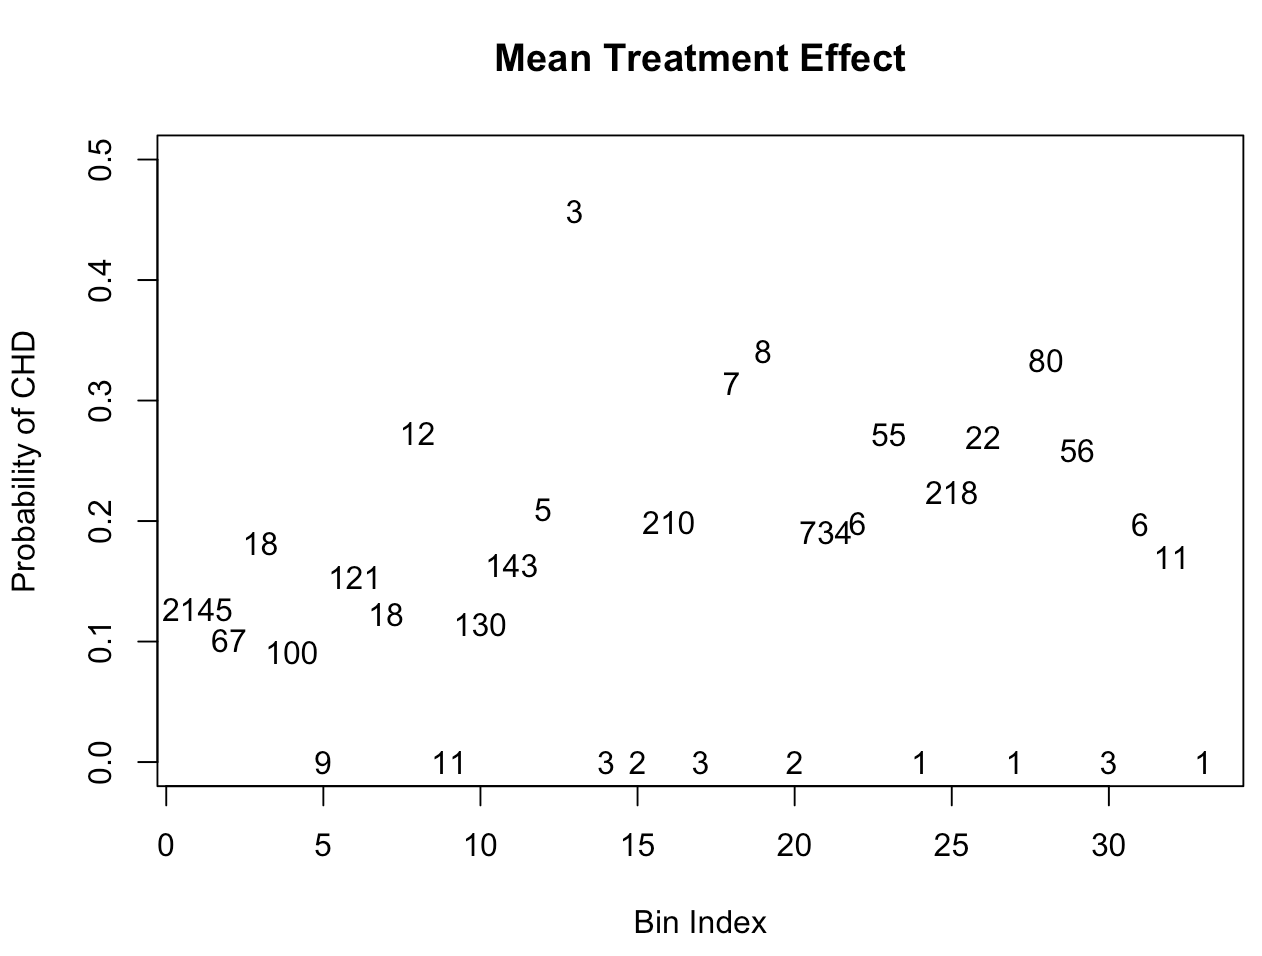
\includegraphics[width=0.5\linewidth]{./effect} 

}

\caption{Expected Outcome}\label{fig:fig5}
\end{figure}

\begin{figure}[H]

{\centering 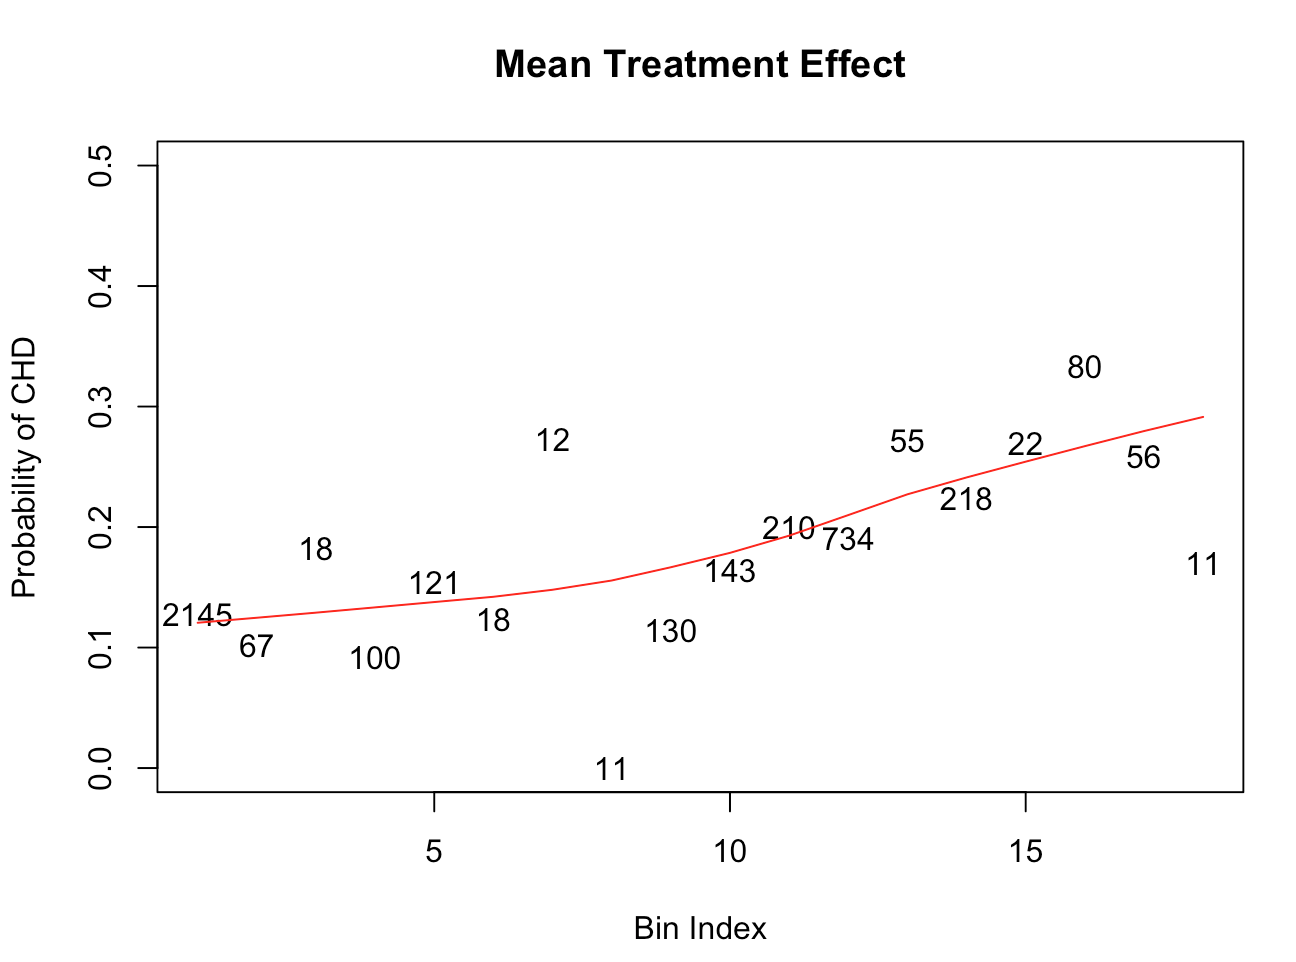
\includegraphics[width=0.5\linewidth]{./pos_violation2} 

}

\caption{Expected Outcome}\label{fig:fig6}
\end{figure}

\newpage

\subsection{Team Member Contribution}\label{team-member-contribution}

\begin{table}[h!]
  \begin{tabular}{|l|l|}
  \hline
    Member & Contributions \\ \hline
    Michael Attah & - group discussion of causal question \\
      & - design of causal graph \\
      & - design of descriptive table \\
      & - categorize covariates: Z\\
      & - interpretation: causal\\ 
      & - references \\ \hline
    Bianca Doone & - group discussion of causal question \\
      & - design of causal graph \\
      & - time-varying assumptions \\
      & - chi-squared test of indepedence\\
      & - categorize covariates: W (age, education, gender) \\
      & - bootstrap confidence intervals: IPTW \\
      & - interpretation: statistical \\
      & - limitations \\ \hline
    Casey Graham & - group discussion of causal question \\
      & - design of causal graph \\
      & - categorize covariates: cigsPerDay \\
      & - computation of simple substitution \\
      & - computation of IPTW \\
      & - computation of Superlearner/TMLE \\ 
      & - bootstrap confidence intervals: TMLE, GLM \\ \hline
    Daniel Saunders & - group discussion of causal question \\
      & - design of causal graph \\
      & - design of descriptive table \\
      & - statistical estimand: G-computation \\
      & - bootstrap confidence intervals: TMLE, simple substitution\\ 
      & - statistical estimand: G-computation \\ \hline
    Nutcha Wattanachit & - group causal question \\
      & - design of causal graph \\
      & - background story and target population \\
      & - specifying causal parameter \\
      & - design of working SCM ($\mathcal{M}^{**}$) \\
      & - specify observed data and link to SCM \\
      & - identifiability: randomization assumption \\
      & - identifiability: positivity assumption \\ \hline
  \end{tabular}
\end{table}

\subsection{References}\label{references}

Boston University \& the National Heart, Lung, \& Blood Institute,
Framingham Heart Study. 5 Dec. 2018:
\url{https://www.framinghamheartstudy.org}

World Health Organization. (2018). Body mass index - BMI. 29 Nov. 2018:
\url{http://www.euro.who.int/en/health-topics/disease-prevention/nutrition/a-healthy-lifestyle/body-mass-index-bmi}

The National Heart, Lung, \& Blood Institute, ATP III Guidelines
At-A-Glance. 29 Nov. 2018:
\url{https://www.nhlbi.nih.gov/files/docs/guidelines/atglance.pdf}


\end{document}
